\chapter{Konzept} \label{section:konzept}

\section{Analyse}

Anfangs soll auf dem Display eine Willkommensnachricht und die bisherige Spielstatistik angezeigt werden. Der Spielablauf beginnt dann mit dem Drücken des Knopfs (im folgenden als Buzzer bezeichnet). In diesem Moment wird die Bombe einem zufälligen Spieler gegeben, der sie dann durch Drücken des Buzzers dem anderen Spieler zuwerfen kann. Nach einer zufälligen Zeit explodiert die Bombe und der Spieler, der sie aktuell hat, verliert diese Runde. Danach wechselt das Spiel zurück in den Startbildschirm und die Statistik wird entsprechend angepasst.

Um obigen Programmablauf realisieren zu können, werden die folgenden Komponenten benötigt:

\begin{itemize}
	\item Timer, für die \zitat{Länge} der Zündschnur
	\item Zufallsgenerator, für die \zitat{Länge} der Zündschnur
	\item LCD Display, zur Darstellung des aktuellen Spielzustandes
	\item Keypad, genauer gesagt ein einziger Knopf zur Steuerung des Spielverlaufs
\end{itemize}

\section{Programmentwurf}

Zur technischen Umsetzung ist der Programmablauf in Abbildung \ref{img:flussdiagramm} geplant.

\begin{figure}[htbp]
	\centering
	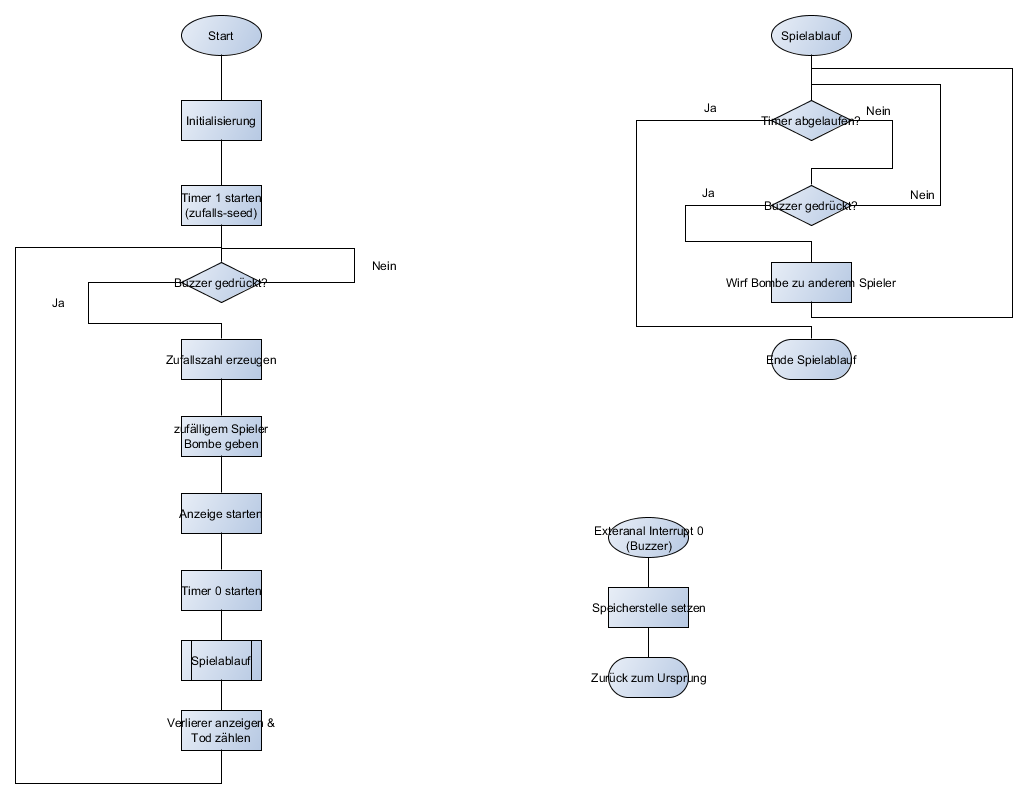
\includegraphics[scale=0.45]{img/Flussdiagramm}
	\caption{Flussdiagramm des Programms}
	\label{img:flussdiagramm}
\end{figure}

Zur Steuerung des Buzzers muss eine Interrupt Routine verwendet werden, um direkt beim Drücken des Buzzers eine Speicherstelle zu setzen. Würde der Buzzer nicht mit einem Interrupt realisiert, könnte es passieren, dass der Spieler den Buzzer bereits wieder losgelassen hat, bevor das Programm an der entsprechenden Verzweigung angekommen ist.

